\scanpage{80}
\mspage{16}
\figure{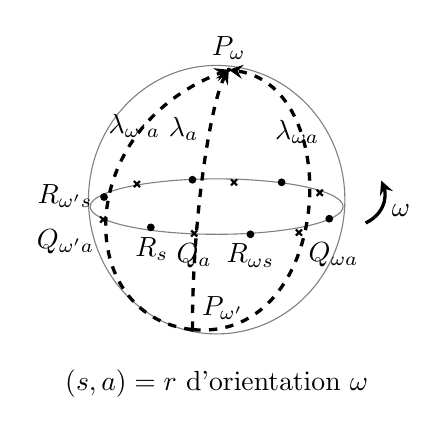
\begin{tikzpicture}[x=1.1cm,y=1.1cm,>=stealth]
\draw[gray,thin] (0,0) ellipse (1.48 and 1.55);
\draw[gray,thin] (0,-0.08) ellipse (1.46 and .32);
\coordinate (N) at (.14,1.5);\coordinate (S) at (-.28,-1.5);
\draw[very thick,dashed,->] (S) .. controls (-1.65,-1.35) and (-1.68,.8) .. (N);
\draw[very thick,dashed,->] (S) .. controls (-.28,-.1) and (-.05,1.17) .. (N);
\draw[very thick,dashed,->] (S) .. controls (1.34,-1.65) and (1.5,1.30) .. (N);
\foreach \x/\y in {-1.3/0.03,-.76/-.32,.39/-.40,1.3/-.22,.75/.20,-.28/.23}
{\fill (\x,\y) circle (.045);}
\foreach \x/\y in {-1.31/-.23,-.26/-.39,.95/-.38,1.19/.08,.20/.20,-.92/.18}
{\draw[thick] (\x-.035,\y-.035)--(\x+.035,\y+.035) (\x-.035,\y+.035)--(\x+.035,\y-.035);}
\fill (N) circle (.025);\fill (S) circle (.025);
\node[above] at (N) {$P_\omega$};\node[above right] at (S) {$P_{\omega'}$};
\node[left] at (-1.32,.04) {$R_{\omega's}$};
\node[below left] at (-1.3,-.23) {$Q_{\omega'a}$};
\node[below] at (-.75,-.32) {$R_s$};
\node[below] at (-.26,-.39) {$Q_a$};
\node[below] at (.39,-.40) {$R_{\omega s}$};
\node[below right] at (.95,-.38) {$Q_{\omega a}$};
\node at (-.95,.85) {$\lambda_{\omega'a}$};
\node at (-.38,.82) {$\lambda_a$};
\node at (.93,.78) {$\lambda_{\omega a}$};
\draw[->,very thick] (1.72,-.27) .. controls (2.00,-.13) and (1.94,.12) .. (1.90,.22);
\node[right] at (1.91,-.13) {$\omega$};
\node[below] at (0,-1.85) {$(s,a)=r$ d'orientation $\omega$};
\end{tikzpicture}}

Je m'intéresse au groupoïde fondamental
\[
\Pi_1(\underbrace{\Sigma_P\setminus S_P}_{\Sigma_P^*\text{ ou }\Sigma^*}),
\]
et je vais écrire d'abord le groupe fondamental en un $P_\omega$, correspondant au choix de $\omega\in\underline\omega$, on pose
\[
(51)\qquad
\underbrace{\Pi_{P,\omega}}_{\text{ou }\Pi_P\text{ ou }\Pi}
=\Pi_1(\Sigma_P^*,P_\omega).
\]
On considère aussi l'opération antiholomorphe unique qui fixe les pts de $\Sigma_{\mathbb R}$, et qui échange $P_\omega$ et $P_{\omega'}$, c'est la conjugaison complexe pour la structure réelle canonique de $\Sigma$, on la note $\tau$.
Ainsi, le groupe
\[
(52)\qquad D_P\times\{1,\tau\}\qquad\text{d'ordre }4n
\]
opère sur $\Sigma$, en respectant la ``carte cyclotomique'' sur $\Sigma$, le sous-groupe qui conserve l'orientation est $D_P$, celui qui induit l'identité sur $S$ (ou sur $P$) est $\{1,\tau\}$. On va aussi \uline{regarder} les groupoïdes fondamentaux mixtes de $\Sigma^*$, pour l'action sur $\Sigma^*$ de $\{1,\tau\}$, de $D_P$, ou de $D_P\times\{1,\tau\}$. \deleted{\unsure{Les groupes sont}}\inserted{On pose}
\[
(53)\qquad
\left\{
\begin{aligned}
\Pi_{P,\omega}^{\tau}&=\Pi_1(\Sigma^*,\{1,\tau\};P_\omega)\\
\Pi_{P,\omega}^{\unsure{D_*|D}}&=\Pi_1(\Sigma^*,D;P_\omega)\\
\Pi_{P,\omega}^{D,\tau}&=\Pi_1(\Sigma^*,D\times\{1,\tau\};P_\omega)
\end{aligned}
\right.
\]
en écrivant aussi $\Pi^\tau,\Pi^D,\Pi^{D,\tau}$ quand $P$ est sous-entendu.
On a donc \deleted{des} un diagramme d'inclusions de
\margin{79}
